%
%
%

\begin{frame}[t,allowframebreaks]{CNN Layer Types: Pooling -}

    In a \index{pooling}\gls{pooling} operation, as in convolution, 
    a \index{filter}\gls{filter} acting on small regions of an input 
    \index{feature map}\gls{feature map}
    is slided over the map with a selected \index{stride}\gls{stride}.\\
    \vspace{0.2cm}

    Unlike the convolution operation which combines 
    all input \glspl{feature map},  
    \index{pooling}\gls{pooling} is {\bf performed 
    at the level of {\em each} \gls{feature map}}.
    \begin{itemize}
        \item 
        \Gls{pooling} {\bf does not change the number of \glspl{feature map}}:
        It produces an output layer with the same depth as the input one.
    \end{itemize}
    \vspace{0.1cm}
    \Gls{pooling} is also referred to as \index{sub-sampling}\gls{sub-sampling}.\\
    \vspace{0.2cm}
    There are several types of \gls{pooling}:
    \begin{itemize}
        \item 
        \index{max pooling}\Gls{max pooling} 
        returns the maximum pixel value within the filter.\\
        In practice, this is the {\bf most common choice}.
        \item 
        \index{average pooling}\Gls{average pooling} 
        returns the average pixel value within the filter.
        \item 
        \index{sum pooling}\Gls{sum pooling} 
        returns the sum of the pixel values within the filter.
        \item 
        \index{stochastic pooling}\Gls{stochastic pooling} 
        returns a random pixel value within the filter.
    \end{itemize}

    \framebreak

    The purpose of \gls{pooling} is to 
    {\bf reduce the size of feature maps} without significant information loss.\\
    \vspace{0.2cm}

    Typically, \index{pooling}\gls{pooling} is run with a 
    \index{stride}\gls{stride} $> 1$ and it can
    {\bf drastically reduce the size} of \index{feature map}\glspl{feature map} 
    without significant information loss.\\

    \begin{center}
        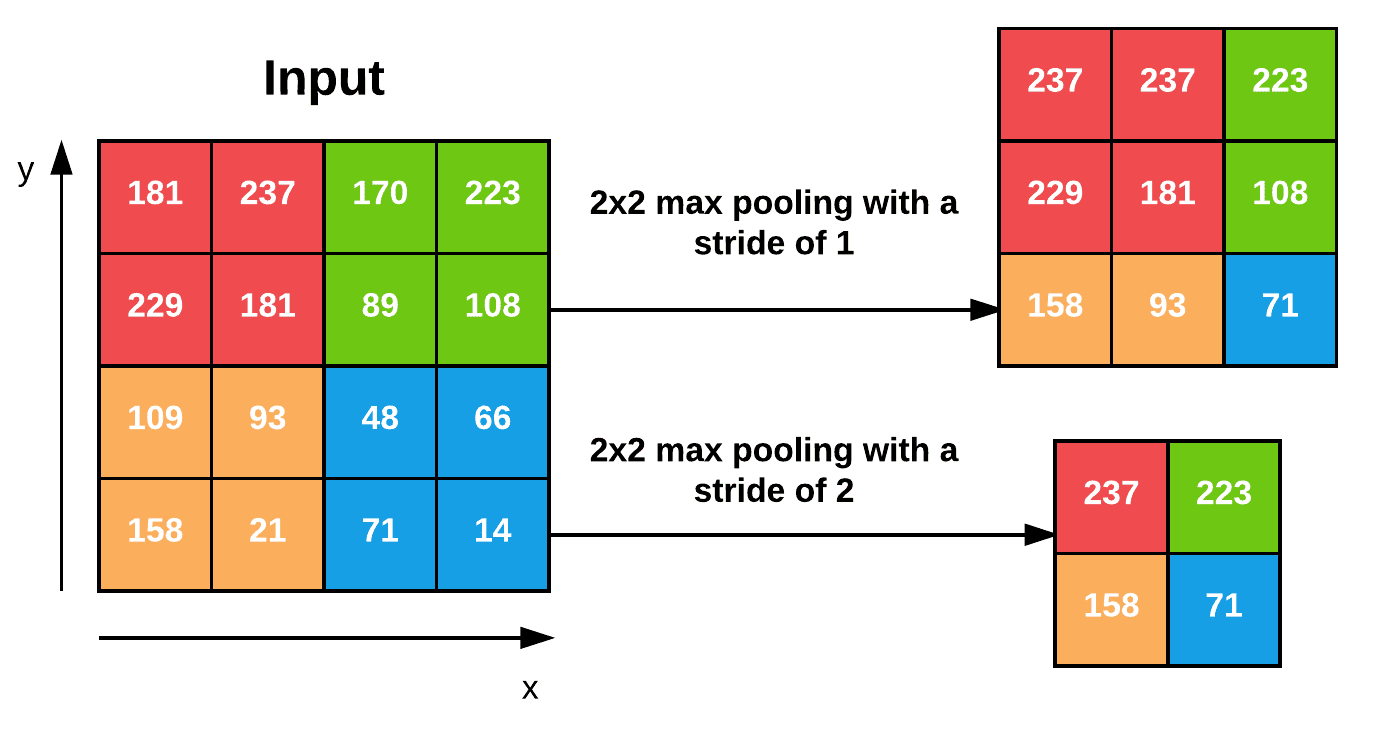
\includegraphics[width=0.70\textwidth]
            {./images/cnn/pooling/rosebrock21_max_pooling_various_strides.png}\\
        \vspace{-0.5cm}
        {\scriptsize
            Example of 2x2 max pooling with different strides.
            \color{col:attribution} 
            Image reproduced from \cite{PyImageSearch:CNNLayerTypes}}\\    
    \end{center}

    \framebreak

    By reducing the spatial resolution of \index{feature map}\glspl{feature map},
    \index{pooling}\gls{pooling} 
    {\bf improves the network 
    \index{translation invariance}translation invariance}.\\
    \vspace{0.2cm}

    \framebreak

    \Gls{pooling} is becoming unpopular and is likely to appear less often in modern 
    network architectures.\\
    \vspace{0.2cm}

    Convolution layers that, occasionally, use large stride can also 
    \begin{itemize}
        \item 
         reduce the size of representations without important information loss,
         \item 
         improve translation invariance, and
        \item 
         introduce non-linearities
    \end{itemize}
    \vspace{0.1cm}

    Architectures replacing \gls{pooling} with 
    convolutional+\gls{relu} layers have achieved similar or better 
    performance using benchmark datasets \cite{Springenberg:2015pl}.\\
    \vspace{0.2cm}

    Removing \gls{pooling} was also found to be important for 
    training stable \glspl{gan} \cite{Radford:2016dcgan}.\\
    \vspace{0.2cm}

    However, other \gls{ml} practitioners have argued that \gls{pooling} can achieve 
    greater translation invariance and that the operation is not
    fully interchangeable with strided convolutions \cite{Aggarwal:2018SpringerDL}.
\end{frame}